% This is "sig-alternate.tex" V2.1 April 2013
% This file should be compiled with V2.5 of "sig-alternate.cls" May 2012
%
% This example file demonstrates the use of the 'sig-alternate.cls'
% V2.5 LaTeX2e document class file. It is for those submitting
% articles to ACM Conference Proceedings WHO DO NOT WISH TO
% STRICTLY ADHERE TO THE SIGS (PUBS-BOARD-ENDORSED) STYLE.
% The 'sig-alternate.cls' file will produce a similar-looking,
% albeit, 'tighter' paper resulting in, invariably, fewer pages.
%
% ----------------------------------------------------------------------------------------------------------------
% This .tex file (and associated .cls V2.5) produces:
%       1) The Permission Statement
%       2) The Conference (location) Info information
%       3) The Copyright Line with ACM data
%       4) NO page numbers
%
% as against the acm_proc_article-sp.cls file which
% DOES NOT produce 1) thru' 3) above.
%
% Using 'sig-alternate.cls' you have control, however, from within
% the source .tex file, over both the CopyrightYear
% (defaulted to 200X) and the ACM Copyright Data
% (defaulted to X-XXXXX-XX-X/XX/XX).
% e.g.
% \CopyrightYear{2007} will cause 2007 to appear in the copyright line.
% \crdata{0-12345-67-8/90/12} will cause 0-12345-67-8/90/12 to appear in the copyright line.
%
% ---------------------------------------------------------------------------------------------------------------
% This .tex source is an example which *does* use
% the .bib file (from which the .bbl file % is produced).
% REMEMBER HOWEVER: After having produced the .bbl file,
% and prior to final submission, you *NEED* to 'insert'
% your .bbl file into your source .tex file so as to provide
% ONE 'self-contained' source file.
%
% ================= IF YOU HAVE QUESTIONS =======================
% Questions regarding the SIGS styles, SIGS policies and
% procedures, Conferences etc. should be sent to
% Adrienne Griscti (griscti@acm.org)
%
% Technical questions _only_ to
% Gerald Murray (murray@hq.acm.org)
% ===============================================================
%
% For tracking purposes - this is V2.0 - May 2012

\documentclass{sig-alternate-05-2015}


\begin{document}

% Copyright
\setcopyright{acmcopyright}
%\setcopyright{acmlicensed}
%\setcopyright{rightsretained}
%\setcopyright{usgov}
%\setcopyright{usgovmixed}
%\setcopyright{cagov}
%\setcopyright{cagovmixed}


% DOI
\doi{10.475/123_4}

% ISBN
\isbn{123-4567-24-567/08/06}

%Conference
\conferenceinfo{PLDI '13}{June 16--19, 2013, Seattle, WA, USA}

\acmPrice{\$15.00}

%
% --- Author Metadata here ---
\conferenceinfo{WOODSTOCK}{'97 El Paso, Texas USA}
%\CopyrightYear{2007} % Allows default copyright year (20XX) to be over-ridden - IF NEED BE.
%\crdata{0-12345-67-8/90/01}  % Allows default copyright data (0-89791-88-6/97/05) to be over-ridden - IF NEED BE.
% --- End of Author Metadata ---

\title{ Mining HIV trends in Social Media Data}
%
% You need the command \numberofauthors to handle the 'placement
% and alignment' of the authors beneath the title.
%
% For aesthetic reasons, we recommend 'three authors at a time'
% i.e. three 'name/affiliation blocks' be placed beneath the title.
%
% NOTE: You are NOT restricted in how many 'rows' of
% "name/affiliations" may appear. We just ask that you restrict
% the number of 'columns' to three.
%
% Because of the available 'opening page real-estate'
% we ask you to refrain from putting more than six authors
% (two rows with three columns) beneath the article title.
% More than six makes the first-page appear very cluttered indeed.
%
% Use the \alignauthor commands to handle the names
% and affiliations for an 'aesthetic maximum' of six authors.
% Add names, affiliations, addresses for
% the seventh etc. author(s) as the argument for the
% \additionalauthors command.
% These 'additional authors' will be output/set for you
% without further effort on your part as the last section in
% the body of your article BEFORE References or any Appendices.

\numberofauthors{2} %  in this sample file, there are a *total*
% of EIGHT authors. SIX appear on the 'first-page' (for formatting
% reasons) and the remaining two appear in the \additionalauthors section.
%
\author{
% You can go ahead and credit any number of authors here,
% e.g. one 'row of three' or two rows (consisting of one row of three
% and a second row of one, two or three).
%
% The command \alignauthor (no curly braces needed) should
% precede each author name, affiliation/snail-mail address and
% e-mail address. Additionally, tag each line of
% affiliation/address with \affaddr, and tag the
% e-mail address with \email.
%
% 1st. author
\alignauthor
Patrick Breen\\
       \affaddr{The Institute of Bioinformatics}\\
       \affaddr{The University of Georgia}\\
       \affaddr{Athens, Georgia}\\
       \email{pbreen@uga.edu}
% 2nd. author
\alignauthor
Shannon Quinn\titlenote{Corresponding author.}\\
       \affaddr{Institute of Computer Science}\\
       \affaddr{University of Georgia}\\
       \affaddr{Athens, Georgia}\\
       \email{squinn@cs.uga.edu}
}



\maketitle
\begin{abstract}

Here is the abstract.

\end{abstract}


%
% The code below should be generated by the tool at
% http://dl.acm.org/ccs.cfm
% Please copy and paste the code instead of the example below. 
%
% TODO: this section
\begin{CCSXML}

\end{CCSXML}


%
% End generated code
%

%
%  Use this command to print the description
%
\printccsdesc

% We no longer use \terms command
%\terms{Theory}

\keywords{ Social Media, Topic Modelling, Document Embedding}

\section{Introduction}

Introduce and literature review of:
1) PrEP, HIV, Twitter


2) Word2Vec, Doc2Vec


3) Dynamic Topic models, Latent Dirichlet allocation


\section{Results}

High level, but more specific than intro, introduce the approach and methods used in this paper here.

\subsection{Word and Document Similarity}

\begin{table}
\centering
\caption{Cosine Similarity to 'prep'}
\begin{tabular}{|l|c|} \hline
Related Word & Cosine Similarity to 'prep'\\ \hline
truvada & 0.836507 \hline
benegative & 0.809185\\ \hline
charliesheen & 0.805214\\ \hline
hivtestweek & 0.797361\\ \hline
sexwork & 0.774867\\ \hline
gettested & 0.765772\\ \hline
hiv & 0.765389\\ \hline
icasa2015 & 0.749948\\ \hline
doingit & 0.749230\\ \hline
aids & 0.738572\\ \hline
\hline\end{tabular}
\end{table}

\begin{table}
\centering
\caption{Cosine Similarity to 'truvada'}
\begin{tabular}{|c|c|} \hline
Related Word & Cosine Similarity to 'truvada'\\ \hline
truvada & 0.836507 \hline
benegative & 0.809185\\ \hline
charliesheen & 0.805214\\ \hline
hivtestweek & 0.797361\\ \hline
sexwork & 0.774867\\ \hline
gettested & 0.765772\\ \hline
hiv & 0.765389\\ \hline
icasa2015 & 0.749948\\ \hline
doingit & 0.749230\\ \hline
aids & 0.738572\\ \hline
\hline\end{tabular}
\end{table}

\subsection{Time Domain}


\begin{figure}
\centering
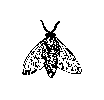
\includegraphics[height=1in, width=1in]{fly}
\caption{Time domain plot.}
\end{figure}


\subsection{User Timeline Analysis}


\subsubsection{Sentiment Classification}



\section{Conclusions}

Conclusions go here.

Example citation (needed right now to compile):\cite{Lamport:LaTeX}

%\end{document}  % This is where a 'short' article might terminate

%ACKNOWLEDGMENTS are optional
\section{Acknowledgments}

Acknowledgements go here.

%
% The following two commands are all you need in the
% initial runs of your .tex file to
% produce the bibliography for the citations in your paper.
\bibliographystyle{abbrv}
\bibliography{sigproc}  % sigproc.bib is the name of the Bibliography in this case
% You must have a proper ".bib" file
%  and remember to run:
% latex bibtex latex latex
% to resolve all references
%
% ACM needs 'a single self-contained file'!
%
% no appendix for now...


\subsection{References}




\end{document}
